\section{Cross-chain event register}
\label{app:case}

The worked case is a single OOv2 request linked to one VotingV2 request. Table~\ref{tab:case_events} locates the five observed endpoints. Full contract addresses, request identifiers, transaction hashes and receipt evidence accompany the register. A log position is interpreted within its transaction and chain; equal-looking identifiers on different chains are not joined without the registered ancillary-data transformation.

\begin{table}[!htbp]
\centering\tabstyle
\caption{Observed endpoints of the worked UMA dispute. UTC coordinates identify actual case events. Explorer links locate the transactions; retained receipts provide the reproducible evidence.}
\label{tab:case_events}
\begin{tabularx}{\linewidth}{@{}L{.22\linewidth}L{.12\linewidth}L{.27\linewidth}Y L{.12\linewidth}@{}}
\toprule Event & Chain & UTC & Block / log & Evidence \\ \midrule
T1 Request & Polygon & 2024-10-29 20:05:50 & 63645613 / 196 & \href{https://polygonscan.com/tx/0x6fc39485f25f23d42bcb55baf68633b31aa5aa53a881116ecf1382e6a1245ede}{Transaction} \\
T2 Proposal & Polygon & 2024-10-30 03:47:16 & 63658346 / 327 & \href{https://polygonscan.com/tx/0xa9ff6827a32b90f134345bbc646a480787676f481ac651b00088520379b47903}{Transaction} \\
T3 Dispute & Polygon & 2024-10-30 03:49:54 & 63658420 / 397 & \href{https://polygonscan.com/tx/0xa5742b4d0b43dbe96de0e57480fbc11a6aa61c64765395db9f27ae45ae5b2198}{Transaction} \\
T4 DVM resolution & Ethereum & 2024-11-03 00:00:35 & 21103395 / 141 & \href{https://etherscan.io/tx/0xc845c4be3da71936e760b5fb8b70eeb8753a7bc5012c452e7d335166d9b14039}{Transaction} \\
T5 Settlement & Polygon & 2024-11-03 00:22:35 & 63813887 / 104 & \href{https://polygonscan.com/tx/0xe9457425a7a67a5e1bb431a7e3b1f8fe4649fcf04f3bb74376caa15600420310}{Transaction} \\
\\[-1.4ex]\bottomrule
\end{tabularx}
\end{table}

The Polygon request, proposal and dispute are decoded from OOv2 events; Ethereum's resolution is decoded from VotingV2. The Polygon settlement retains the same resolved value. Native request hashing and ancillary-data transformations support the identity match. The five retained transactions do not provide a complete sequence of relay acceptance, processing and return operations, so the interval between dispute and resolution is not attributed solely to voting or solely to transport.

\begin{figure}[!htbp]
\centering
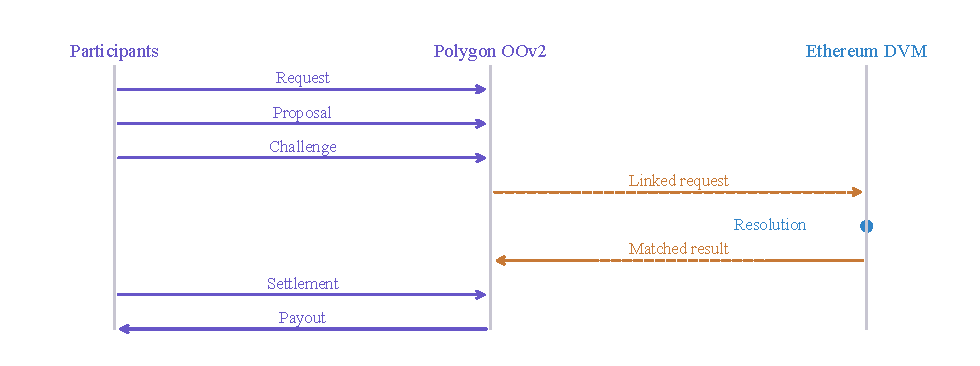
\includegraphics[width=0.99\linewidth]{figures/cross_chain_evidence_links.pdf}
\caption{Evidence links in the worked case. Solid arrows denote observed participant actions or transfers. Dashed arrows connect matched request identities and outcomes across chains; they do not represent an independently reconstructed relay path. Vertical order is schematic. Elapsed times are shown in Figure~\ref{fig:case}.}
\label{fig:cross_chain_links}
\end{figure}

Accounting separates both deposits, the winner's gross payout and the protocol fee. Principal return and gain decompose one payout and must not be added again as transfers. The configured reward is tracked separately. Early expiration retains its native meaning; the proposition lacks independent factual adjudication.
